%%%%%%%%%%%%%%%%%%%%%%%%%%%%%%%%%%%%%%%%%%%%%%%%%%%%%%%%%%%%%%%%%%%%%%%%%%%%%%%
% Chapter 3: Procedimiento experimental 
%%%%%%%%%%%%%%%%%%%%%%%%%%%%%%%%%%%%%%%%%%%%%%%%%%%%%%%%%%%%%%%%%%%%%%%%%%%%%%%



%++++++++++++++++++++++++++++++++++++++++++++++++++++++++++++++++++++++++++++++
\section{Descripci�n de los experimentos}
\label{3:sec:1}

En este apartado se explicar� el procedimiento que se ha seguido para la resoluci�n de 
la integral definida de la funci�n $f(x)=x^{2}\ cos\ x$ en el intervalo acotado $[1,3]$
utilizando el segundo teorema fundamental del c�lculo integral (o Regla de Barrow) para 
calcular f�cilmente el valor de la integral definida a partir de cualquiera de las 
primitivas de la funci�n.

Una vez obtenido el valor de la integral de la funci�n, se proceder� a la aplicaci�n de 
la Regla de Simpson para obtener una aproximaci�n de dicha integral y comparar as� ambos 
resultados.

\subsection{C�lculo del valor de la integral definida}

A continuaci�n se detallar�n los pasos seguidos para obtener el valor exacto de la 
integral definida.

Se quiere calcular:

\[ \int_{1}^{3} x^2\ cos\ x\ \text{d}x \]

Primero se resuelve la integral indefinida aplicando el m�todo de integraci�n por 
partes 
$\left(\int u \text{d}v = uv - \int v \text{d}u\right)$ tal que:

\[ u=x^2, \quad \text{d}u = 2x \text{d}x \]
\[ \text{d}v = cos\ x \text{d}x, \quad v = sen\ x \]

Con lo que se obtiene:

\[ \int x^2\ cos\ x\ \text{d}x = x^2 sen\ x - \int 2x sen\ x \text{d}x = \]

Empleando de nuevo la integraci�n por partes:

\[ u=2x, \quad \text{d}u = 2 \text{d}x \]
\[ \text{d}v = sen\ x \text{d}x, \quad v = -cos\ x \]

Se sigue:

\[ = x^2 sen\ x - \left[-2x cos\ x + 2\int cos\ x\ \text{d}x \right] = 
x^2 sen\ x +2x cos\ x - 2sen\ x = \]

\begin{equation}
 2x cos\ x + (x^2 -2)sen\ x
 \label{ec1}
\end{equation}

Por �ltimo se obtiene el valor buscado a trav�s de la Regla de Barrow en el 
intervalo $[1,3]$. Para ello se emplear� el lenguaje de programaci�n interpretado
Python, a trav�s de una funci�n que eval�a la expresi�n ~\ref{ec1}. 

\subsection{Aproximaci�n por la Regla de Simpson}

Para el c�lculo de una aproximaci�n de la integral:

\[ \int_{1}^{3} x^2\ cos\ x\ \text{d}x \]

se emplea el lenguaje Python implementando una funci�n que recibe por 
par�metros la expresi�n a estudiar y lo extremos del intervalo donde se va a calcular, 
devolviendo la aproximaci�n buscada. (Ver Ap�ndice 1).

\subsection{Aproximaci�n por la Regla de Simpson Compuesta}

Para un mejor an�lisis de los resultados, se repite el estudio aplicando la Regla de 
Simpson Compuesta, implementando una funci�n en Python que recibe por par�metros la expresi�n a estudiar. 
los extremos del intervalo y el n�mero de subintervalos en los que se ha dividido, devolviendo la 
aproximaci�n buscada. (Ver Ap�ndice 1)

\subsection{Comparativa de Resultados}
Para finalizar el experimento se realiza una comparativa de las aproximaciones obtenidas a trav�s de la 
Regla de Simpson con el valor exacto de la funci�n $f(x)$ objeto de estudio en el intervalo dado.

Como puede verse en el Ap�ndice 2, se implementa un programa en Python que muestra por pantalla los errores 
absolutos y relativos de cada experimento.


%++++++++++++++++++++++++++++++++++++++++++++++++++++++++++++++++++++++++++++++
\section{Descripci�n del material}
\label{3:sec:2}
Las caracter�sticas del ordenador empleado para la realizaci�n de este trabajo son las siguientes:
\begin{itemize}
 \item CPU type: Intel(R) Atom(TM) CPU N270   @ 1.60GHz
 \item CPU speed: 800.000Hz
 \item Cache size: 512 KB
\end{itemize}
En cuanto al sistema operativo, se ha utlizado ``Linux-3.2.0-39-generic-i686-with-Ubuntu-12.04-precise''.
Los ficheros en lenguaje Python fueron realizados con el editor de textos avanzado para KDE ``Kate''.

%++++++++++++++++++++++++++++++++++++++++++++++++++++++++++++++++++++++++++++++
\section{Resultados obtenidos}
\label{3:sec:3}

%------------------------------------------------------------------------------
\begin{figure}[!th]
\begin{center}
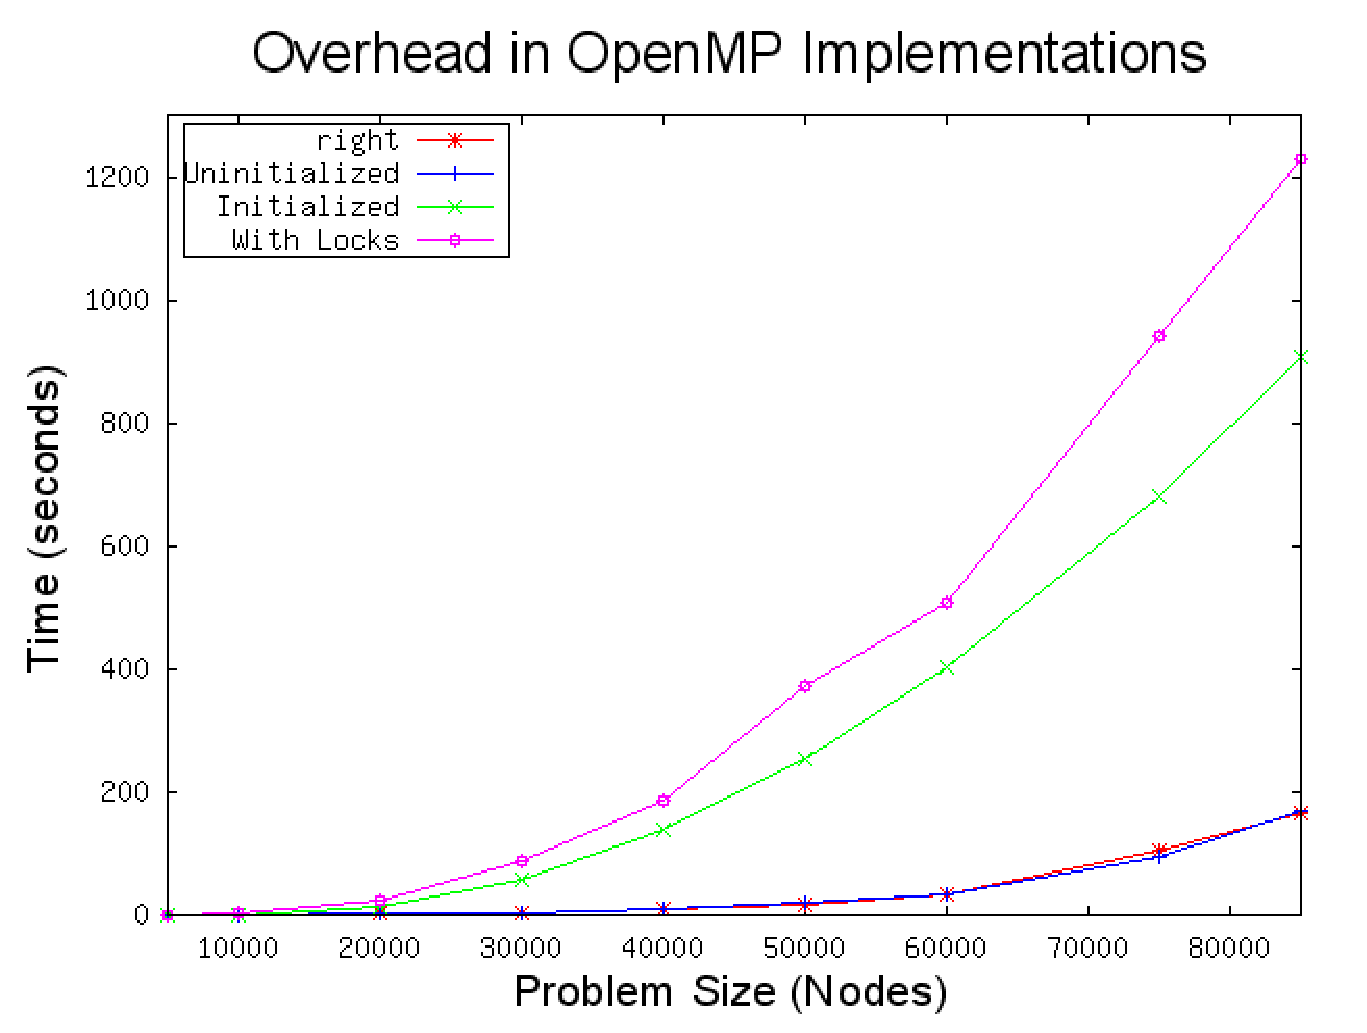
\includegraphics[width=0.75\textwidth]{images/figura1.eps}
\caption{Ejemplo de figura}
\label{fig:1}
\end{center}
\end{figure}
%------------------------------------------------------------------------------
%--------------------------------------------------------------------------
\begin{table}[h]
\begin{center}
\begin{tabular}{|c|c|c|c|} \hline 
\textbf{Valor exacto} & \textbf{Aproximacion} & \textbf{Error absoluto} & \textbf{Error relativo}\\ 
\hline
-5.19124855011 & -5.0093265161 & 0.181922034015 & 0.0350439845558
\\
\hline
\end{tabular}
\end{center}
\caption{Aproximacion y error de la regla de Simpson}
\label{tab:1}
\end{table}


%------------------------------------------------------------------------------
%--------------------------------------------------------------------------
\begin{table}[h]
  \begin{center}
    \begin{tabular}{|c|c|c|c|c|} \hline 
      \textbf{N\'umero de subintervalos} & \textbf{Aproximaci\'on} & \textbf{Error absoluto} & \textbf{Error relativo}\\ 
      \hline
      2 & -5.1817934049 & 0.0094551452 & 0.0018213625
      \\
      \hline
      6 & -5.1911377092 & 0.0001108409 & 0.0000213515
      \\
      \hline
      10 & -5.1912342437 & 0.0000143064 & 0.0000027559
      \\
      \hline
      50 & -5.1912485273 & 0.0000000228 & 0.0000000044
      \\
      \hline
      100 & -5.1912485487 & 0.0000000014 & 0.0000000003
      \\
      \hline
    \end{tabular}
  \end{center}
  \caption{Aproximaci\'on y error de la regla de Simpson compuesta}
  \label{tab:2}
\end{table}


%++++++++++++++++++++++++++++++++++++++++++++++++++++++++++++++++++++++++++++++

\section{An�lisis de los resultados}
\label{3:sec:4}

bla, bla, etc. 

